\سؤال{}

یک ساعت دیجیتال معمولی را در نظر می‌گیریم.

\begin{itemize}
	\item الف)
	\begin{itemize}
		\item اتکاپذیری:
			\begin{itemize}
				\item دسترس‌پذیری:
				 باید هر زمان که از ساعت می‌خواهیم استفاده کنیم، کار کند.
				 \item قابلیت اطمینان:
				 باید زمان را به درستی نشان دهد. 
				 \item امنیت:
				 این ویژگی در ساعت اهمیت چندانی ندارد.
				\item قابلیت نگهداری:
				 باید بتوان از ساعت دیجیتال به درستی نگهداری کرد و قطعات آن در بازار موجود باشد.  
			\end{itemize}
		\item مصرف انرژی: مصرف انرژی آن باید تا حد امکان کم باشد.
		\item کارایی:
		اگر کارایی را مطابق با فرمول زیر در نظر بگیریم، باید کارایی آن ۱ باشد. 
		$$performance = \frac{1}{execution\: time}$$
		\item وزن:
		نباید وزن زیادی داشته باشد.
		\item قیمت:
		هزینه‌ی ساخت آن نباید زیاد شود.
		\item سایز کد:
		نباید کد اجرای آن  بزرگ شود،تا از قطعات کم‌تری استفاده شود. 
		\item همان‌طور که در سایز کد گفته شد، باید از کم‌ترین منابع با بیش‌ترین قدرت استفاده کرد.
		\item بی‌درنگ:
		چون کاربرد آن استفاده تشخیص زمان است، بنابراین، محدودیت بی‌درنگ بودن در آن از اهمیت بالایی برخوردار است.
	\end{itemize}
	\item ب)
	\begin{figure}[!hbpt]
		\centering
		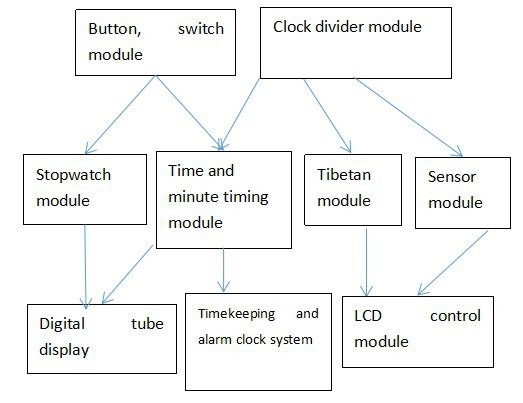
\includegraphics[scale=0.6]{img/a.jpeg}
		\caption{نمودار بلوکی ساعت دیجیتال}
	\end{figure}
	\item ج) 
	اگر در این قسمت قیمت‌ تمام شده را در نظر بگیریم، چه برای شرکت تولیدکننده چه برای تولید شخصی محصول، اختلاف قیمت وجود خواهد شد. دلیل وجود این اختلاف قیمت، حذف شدن هزینه‌ی طراحی اولیه و مهندسی (که در سوال ۳ راجع‌به آن توضیح داده شده است) می‌باشد. به همین دلیل قیمت برای شرکت تولیدکننده کم‌تر از تولید آن با جنس، کیفیت و ... مشابه همان محصول به طور شخصی است.
	
\end{itemize}
